\documentclass[12pt, a4paper]{report}

% ======================================================================
% PREAMBLE: PACKAGES & SETTINGS (same format as the reference report)
% ======================================================================
\usepackage[utf8]{inputenc}
\usepackage[T1]{fontenc}
\usepackage{geometry}
\geometry{a4paper, left=1.9cm, right=1.9cm, top=2.5cm, bottom=1.9cm, headheight=15pt, headsep=0.6cm, includefoot}
\usepackage{graphicx}
\usepackage{hyperref}
\usepackage{fancyhdr}
\usepackage{titlesec}
\usepackage{setspace}
\usepackage{tabularx}
\usepackage{eso-pic}
\usepackage[expansion=false,protrusion=false]{microtype}
\usepackage{listings}
\usepackage{xcolor}
\usepackage{booktabs}
\usepackage{float}
\usepackage{seqsplit}
\usepackage{tikz}
\usepackage{pgfplots}
\usetikzlibrary{calc, shapes.geometric, arrows.meta, positioning, fit, backgrounds, decorations.pathreplacing}
\pgfplotsset{compat=1.18}

\onehalfspacing

\tolerance=10000
\hbadness=10000
\emergencystretch=3em

\hypersetup{
    colorlinks=true,
    linkcolor=black,
    filecolor=black,
    urlcolor=blue,
    pdftitle={Project Report - Recall AI Quiz Studio},
}

% ---------- code listing styles ----------
\lstset{
    basicstyle=\ttfamily\footnotesize,
    breaklines=true,
    breakatwhitespace=false,
    postbreak=\mbox{\textcolor{gray}{$\hookrightarrow$}\space},
}
\lstdefinelanguage{JSON}{
    basicstyle=\ttfamily\footnotesize,
    showstringspaces=false,
    breaklines=true,
    frame=single,
    backgroundcolor=\color{gray!5},
    rulecolor=\color{gray!40},
}
\lstdefinestyle{pseudo}{
    basicstyle=\ttfamily\footnotesize,
    keywordstyle=\bfseries\color{blue},
    commentstyle=\itshape\color{green!50!black},
    stringstyle=\color{orange},
    breaklines=true,
    frame=single,
    backgroundcolor=\color{gray!5},
    rulecolor=\color{gray!40},
}

% ---------- page border on every page ----------
\AddToShipoutPictureBG{%
\begin{tikzpicture}[overlay,remember picture]
\draw[line width=1.5pt]
    ($(current page.north west) + (0.7cm,-0.7cm)$)
    rectangle
    ($(current page.south east) + (-0.7cm,0.7cm)$);
\end{tikzpicture}
}

% ======================================================================
% PLACEHOLDERS - edit these once, they are used on every front page
% ======================================================================
\newcommand{\ProjectTitle}{Recall: AI Quiz Studio}
\newcommand{\GuideName}{[Guide Name]}
\newcommand{\GuideDesignation}{[Guide Designation]}
\newcommand{\SubmissionMonth}{[Month Year]}
\newcommand{\SubmissionDate}{[DD/MM/YYYY]}
\newcommand{\MemberOne}{[Student Name 1]}   \newcommand{\RollOne}{[Roll No. 1]}
\newcommand{\MemberTwo}{[Student Name 2]}   \newcommand{\RollTwo}{[Roll No. 2]}
\newcommand{\MemberThree}{[Student Name 3]} \newcommand{\RollThree}{[Roll No. 3]}
\newcommand{\MemberFour}{[Student Name 4]}  \newcommand{\RollFour}{[Roll No. 4]}

% ---------- screenshot slot ----------
% \screenshot[width]{file-name-without-extension}{caption}{label}{what to capture}
% If report/images/screenshots/<file>.png (or .jpg) exists it is shown,
% otherwise a dashed placeholder box describing what to capture is drawn.
\newcommand{\screenshot}[5][0.85]{%
\begin{figure}[H]
\centering
\IfFileExists{images/screenshots/#2.png}{%
    \includegraphics[width=#1\textwidth,height=0.36\textheight,keepaspectratio]{images/screenshots/#2.png}}{%
\IfFileExists{images/screenshots/#2.jpg}{%
    \includegraphics[width=#1\textwidth,height=0.36\textheight,keepaspectratio]{images/screenshots/#2.jpg}}{%
    \begin{tikzpicture}
    \node[draw=gray, dashed, thick, minimum width=#1\textwidth, minimum height=4.6cm,
          align=center, text width=#1\textwidth-1cm, fill=gray!6, font=\small]
          {\textbf{[ SCREENSHOT PLACEHOLDER ]}\\[2pt] \texttt{images/screenshots/\detokenize{#2}.png}\\[4pt] \textit{#5}};
    \end{tikzpicture}}}
\caption{#3}
\label{#4}
\end{figure}
}

\begin{document}
\sloppy

% ======================================================================
% TITLE PAGE
% ======================================================================
\begin{titlepage}
\centering
\vspace*{0.2cm}
{\Large \textbf{A PROJECT REPORT}}\\[0.3cm]
{\large \textbf{on}}\\[0.3cm]
{\LARGE \textbf{``\ProjectTitle''}}\\[0.5cm]
{\large Submitted to}\\[0.1cm]
{\large \textbf{KIIT Deemed to be University}}\\[0.4cm]
{\large In Partial Fulfilment of the Requirement for the Award of}\\[0.2cm]
{\Large \textbf{BACHELOR'S DEGREE IN}}\\[0.1cm]
{\Large \textbf{COMPUTER SCIENCE AND ENGINEERING}}\\[0.5cm]
{\large \textbf{BY}}\\[0.3cm]
{\large
\begin{center}
\begin{tabular}{@{} l @{\hspace{2cm}} l @{}}
\textbf{\MemberOne}   & \textbf{\RollOne} \\
\textbf{\MemberTwo}   & \textbf{\RollTwo} \\
\textbf{\MemberThree} & \textbf{\RollThree} \\
\textbf{\MemberFour}  & \textbf{\RollFour} \\
\end{tabular}
\end{center}
}
\vspace{0.3cm}
\vfill
{\large \textbf{UNDER THE GUIDANCE OF}}\\[0.2cm]
{\large \textbf{\GuideName}}\\[0.4cm]

\includegraphics[width=0.25\textwidth]{images/KIIT_logo.png}\\[0.4cm]
{\large \textbf{SCHOOL OF COMPUTER ENGINEERING}}\\[0.1cm]
{\large \textbf{KALINGA INSTITUTE OF INDUSTRIAL TECHNOLOGY}}\\[0.1cm]
{\large \textbf{BHUBANESWAR, ODISHA - 751024}}\\[0.3cm]
{\large \textbf{\SubmissionMonth}}
\end{titlepage}

\pagenumbering{roman}
\setcounter{page}{2}

% ======================================================================
% CERTIFICATE
% ======================================================================
\phantomsection
\addcontentsline{toc}{chapter}{Certificate}
\begin{center}
{\Large \textbf{KIIT Deemed to be University}}\\[0.2cm]
{\large \textbf{School of Computer Engineering}}\\[0.2cm]
{\large \textbf{Bhubaneswar, ODISHA 751024}}\\[0.8cm]

\includegraphics[width=0.20\textwidth]{images/KIIT_logo.png}\\[0.8cm]
{\LARGE \textbf{CERTIFICATE}}\\[1cm]
\end{center}

This is to certify that the project report entitled \textbf{``\ProjectTitle''} is a bona fide record of work carried out by \textbf{\MemberOne}, \textbf{\MemberTwo}, \textbf{\MemberThree}, and \textbf{\MemberFour} under my supervision and guidance, in partial fulfilment of the requirements for the award of the Degree of Bachelor's in Computer Science and Engineering from KIIT Deemed to be University, Bhubaneswar.

\vfill
\noindent
\begin{minipage}[t]{0.45\textwidth}
\vspace{2cm}
\textbf{Date:} \SubmissionDate
\end{minipage}\hfill
\begin{minipage}[t]{0.5\textwidth}
\raggedleft
\textbf{Signature of Guide}\\[1cm]
\textbf{\GuideName}\\[0.2cm]
\GuideDesignation\\
School of Computer Engineering\\
KIIT Deemed to be University
\end{minipage}
\vspace*{1cm}

% ======================================================================
% DECLARATION
% ======================================================================
\newpage
\phantomsection
\addcontentsline{toc}{chapter}{Declaration}
\begin{center}
{\LARGE \textbf{DECLARATION}}\\[1cm]
\end{center}

We hereby declare that the project report entitled \textbf{``\ProjectTitle''} submitted to KIIT Deemed to be University, Bhubaneswar, in partial fulfilment of the requirements for the award of the Degree of Bachelor's in Computer Science and Engineering, is a record of original work carried out by us.

\vfill
\noindent
\begin{minipage}[b]{0.4\textwidth}
\textbf{Place:} Bhubaneswar\\[0.3cm]
\textbf{Date:} \SubmissionDate
\end{minipage}\hfill
\begin{minipage}[b]{0.6\textwidth}
\raggedleft
\textbf{\MemberOne} (\dots\dots\dots\dots\dots\dots)\\[0.2cm]
\textbf{\MemberTwo} (\dots\dots\dots\dots\dots\dots)\\[0.2cm]
\textbf{\MemberThree} (\dots\dots\dots\dots\dots\dots)\\[0.2cm]
\textbf{\MemberFour} (\dots\dots\dots\dots\dots\dots)
\end{minipage}
\vspace*{1cm}

% ======================================================================
% ACKNOWLEDGEMENT
% ======================================================================
\newpage
\phantomsection
\addcontentsline{toc}{chapter}{Acknowledgement}
\begin{center}
{\LARGE \textbf{ACKNOWLEDGEMENT}}\\[1cm]
\end{center}

We would like to express our profound gratitude to our project guide, \textbf{\GuideName}, for their valuable guidance, continuous encouragement, and invaluable support throughout the development of this project.

\par\vspace{0.5cm}
We also extend our sincere thanks to the Head of the Department, School of Computer Engineering, KIIT Deemed to be University, for providing us with the necessary facilities and a conducive environment to carry out this work.

\vfill
\begin{flushright}
\textbf{\MemberOne\ (\RollOne)}\\[0.15cm]
\textbf{\MemberTwo\ (\RollTwo)}\\[0.15cm]
\textbf{\MemberThree\ (\RollThree)}\\[0.15cm]
\textbf{\MemberFour\ (\RollFour)}
\end{flushright}
\vspace*{1cm}

% ======================================================================
% ABSTRACT
% ======================================================================
\newpage
\phantomsection
\addcontentsline{toc}{chapter}{Abstract}
\begin{center}
{\LARGE \textbf{ABSTRACT}}\\[1cm]
\end{center}

Preparing practice questions is slow, and most self-study tools either ship a fixed question bank or ask the learner to write every question by hand. This project presents \textbf{Recall}, a locally hosted web application that turns \textit{any topic} or \textit{any uploaded study material} into a complete quiz within seconds. A learner can type a topic such as ``Dijkstra's algorithm'', or upload PDF, DOCX, PPTX, TXT and Markdown files, choose Easy, Medium or Hard difficulty, and receive a mix of multiple-choice, written-answer and coding questions.

\par\vspace{0.5cm}
The system is built as a Flask JSON API with a framework-free HTML, CSS and JavaScript single-page front end. For topic quizzes, a research module gathers source text in parallel from Wikipedia, DuckDuckGo and, optionally, the Tavily search API, so that questions are grounded in real sources that are listed on the results page. Question generation is delegated to a large language model through a pluggable engine layer: the Groq cloud API is used when an API key is configured, and a local Ollama model acts as an offline fallback. Every model reply is parsed and validated against a strict JSON schema, and a retry-with-fallback loop protects the user from malformed output. Written answers are graded by the language model against a model answer and a list of key points, and coding answers are executed against test cases in a time-limited subprocess sandbox. The interface offers a Practice mode with instant feedback and a timed Exam mode with a question grid and review flags, a retry-mistakes loop, history and statistics stored in the browser, and JSON and Markdown export.

\par\vspace{0.5cm}
This report documents the requirements, architecture, API design, AI generation pipeline, research and ingestion modules, code sandbox, front end, security considerations, testing and future scope of the system.

\par\vspace{0.5cm}
\noindent\textbf{Keywords:} Quiz Generation, Large Language Model, Prompt Engineering, Retrieval of Web Sources, Automated Grading, Document Processing, Flask, Groq, Ollama, Single-Page Application.

% ======================================================================
% PROJECT CONTRIBUTORS
% ======================================================================
\newpage
\phantomsection
\addcontentsline{toc}{chapter}{Project Contributors}
\begin{center}
{\LARGE \textbf{PROJECT CONTRIBUTORS}}\\[0.8cm]
\end{center}

\noindent \textbf{1. Technical Implementation \& Engineering Contributions} \\
The primary technical responsibilities of each member are outlined below.
\begin{itemize}
\item \setlength{\itemsep}{0pt}\textbf{\MemberOne:} [Describe technical contribution, e.g.\ backend API and AI engine integration.]
\item \setlength{\itemsep}{0pt}\textbf{\MemberTwo:} [Describe technical contribution, e.g.\ front-end single-page application.]
\item \setlength{\itemsep}{0pt}\textbf{\MemberThree:} [Describe technical contribution, e.g.\ web research and document ingestion.]
\item \setlength{\itemsep}{0pt}\textbf{\MemberFour:} [Describe technical contribution, e.g.\ code sandbox, testing and deployment.]
\end{itemize}
\vspace*{0.3cm}
\noindent \textbf{2. Individual Contribution to Project Report Preparation} \\
Documentation responsibilities were partitioned to match each member's technical domain.
\begin{itemize}
\item \setlength{\itemsep}{0pt}\textbf{\MemberOne:} [Chapters authored.]
\item \setlength{\itemsep}{0pt}\textbf{\MemberTwo:} [Chapters authored.]
\item \setlength{\itemsep}{0pt}\textbf{\MemberThree:} [Chapters authored.]
\item \setlength{\itemsep}{0pt}\textbf{\MemberFour:} [Chapters authored.]
\end{itemize}

% ======================================================================
% CONTENTS, FIGURES, TABLES, ABBREVIATIONS
% ======================================================================
\newpage
\tableofcontents
\newpage
\listoffigures
\addcontentsline{toc}{chapter}{List of Figures}
\newpage
\listoftables
\addcontentsline{toc}{chapter}{List of Tables}

\newpage
\phantomsection
\addcontentsline{toc}{chapter}{List of Abbreviations}
\begin{center}
{\LARGE \textbf{LIST OF ABBREVIATIONS}}\\[1cm]
\end{center}
\begin{tabularx}{\textwidth}{@{} p{3cm} X @{}}
\toprule
\textbf{Abbreviation} & \textbf{Full Form} \\
\midrule
AI & Artificial Intelligence \\
API & Application Programming Interface \\
CSS & Cascading Style Sheets \\
DFD & Data Flow Diagram \\
DOCX / PPTX & Microsoft Word / PowerPoint Open XML formats \\
HTML & HyperText Markup Language \\
HTTP & HyperText Transfer Protocol \\
IEEE & Institute of Electrical and Electronics Engineers \\
JSON & JavaScript Object Notation \\
LLM & Large Language Model \\
MCQ & Multiple-Choice Question \\
PDF & Portable Document Format \\
REST & Representational State Transfer \\
SPA & Single-Page Application \\
SRS & Software Requirements Specification \\
UI / UX & User Interface / User Experience \\
WSGI & Web Server Gateway Interface \\
\bottomrule
\end{tabularx}

% ======================================================================
% MAIN MATTER
% ======================================================================
\newpage
\pagenumbering{arabic}

\chapter{Introduction}

\section{Overview and Background}
Active recall, the practice of retrieving information from memory instead of simply re-reading it, is one of the most effective study techniques available to students. Quizzes are its most natural form. In practice, however, learners rarely have a quiz that matches exactly what they are studying: published question banks are generic, and writing good questions manually, with plausible wrong options, model answers and test cases, takes longer than studying the material itself.

Recent large language models (LLMs) can read a passage and produce well-formed questions about it. The remaining engineering problem is to make this reliable and useful: the model must be given trustworthy source material, its output must be forced into a machine-readable structure, the answers must be graded, and the whole experience must feel like a quiz and not a chat window.

\textbf{Recall} is a web application that addresses this problem. A learner either types a topic or uploads study material, chooses a difficulty and a question mix, and receives a ready-to-take quiz containing multiple-choice, written and coding questions. The application runs on the learner's own machine, so uploaded notes never have to be stored on a third-party server other than the model provider that is explicitly selected.

\section{Problem Statement}
Students preparing for examinations face the following recurring difficulties:
\begin{itemize}
\item Ready-made question banks do not cover the learner's own notes, slides or syllabus.
\item Writing questions, distractors, model answers and test cases manually is time-consuming.
\item Asking a general chat assistant for ``a quiz'' produces free-form text that cannot be taken, scored, timed or reviewed inside an application.
\item Questions invented by a model without source material may contain factual errors, and the learner has no way to see where a question came from.
\item Written and coding answers need feedback, which most static quiz tools cannot give.
\end{itemize}
There is therefore a need for a single tool that generates \textit{grounded}, \textit{structured} and \textit{gradable} quizzes from arbitrary topics and documents.

\section{Objectives of the System}
The objectives of the project are:
\begin{enumerate}
\item To generate quizzes on any user-typed topic, grounded in web sources whose names and links are shown to the learner.
\item To generate quizzes from uploaded PDF, DOCX, PPTX, TXT and Markdown files and from pasted text.
\item To support three question types (multiple choice, written answer and coding) at Easy, Medium and Hard difficulty.
\item To enforce a strict JSON schema on model output and to recover automatically from malformed or empty replies.
\item To provide two engines, a fast cloud engine (Groq) and an offline local engine (Ollama), with automatic fallback.
\item To grade written answers with AI feedback and to execute coding answers against test cases.
\item To provide Practice mode (instant feedback) and Exam mode (timer, question grid, flag for review), together with history, statistics and export.
\end{enumerate}

\section{Scope and Limitations}
\textbf{Scope.} The system covers quiz generation, taking, grading, reviewing and exporting for a single learner using a modern desktop or mobile browser. It includes the Flask back end, the research and document-ingestion modules, the code sandbox and the single-page front end.

\textbf{Limitations.}
\begin{itemize}
\item The system depends on the quality of the selected language model; the small local model gives noticeably weaker questions than the cloud model.
\item Quiz history is stored only in the browser's local storage; there are no user accounts and no cross-device synchronisation.
\item The code runner executes Python only, and it runs submitted code in a plain subprocess on the host machine. It is intended for local, single-user use and is not a hardened multi-tenant sandbox.
\item Scanned PDFs without a text layer cannot be read, because no optical character recognition is performed.
\item The project does not currently include an automated test suite; testing was performed manually (Chapter~\ref{chap:security}).
\end{itemize}

\chapter{Literature Review}

\section{Introduction}
This chapter surveys the categories of tools and techniques that Recall builds on: existing quiz and flash-card platforms, automatic question generation, grounding language models with retrieved text, automated grading of free-text answers, and automatic assessment of programming exercises. The discussion is deliberately descriptive; formal citations should be added to the bibliography by the authors from the sources they consulted.

\section{Existing Quiz and Study Platforms}
Flash-card and quiz platforms such as Quizlet, Kahoot and Google Forms quizzes let a teacher or learner author question sets and then deliver them with scoring, timers and sharing. Their strength is polished delivery; their weakness is that \textit{every question must be written by a human}. Learning-management systems offer large question banks, but these are tied to a specific course and rarely match a learner's own notes.

\section{Automatic Question Generation}
Automatic question generation (AQG) has been studied for many years, first with rule-based and template-based systems that transform sentences into questions, and later with neural sequence-to-sequence models. Template approaches produce grammatical but shallow questions. Modern instruction-tuned LLMs can write multi-sentence stems, plausible distractors and explanations in a single pass, and can be asked to adjust cognitive level. Recall uses this capability and expresses the target level through a per-difficulty guidance string (recall of facts for Easy, application for Medium, multi-step analysis for Hard).

\section{Grounding Language Models with Retrieved Text}
A known weakness of LLMs is \textit{hallucination}: fluent statements that are not true. A widely used mitigation is to retrieve relevant text first and instruct the model to answer only from it. Recall applies this idea in two ways. For document quizzes the uploaded text is the grounding material. For topic quizzes, a research module retrieves plain-text extracts from Wikipedia, a DuckDuckGo abstract and, optionally, Tavily search results, then asks the model to quote the supporting passage for each multiple-choice question in a \texttt{source\_quote} field.

\section{Automated Grading of Written Answers}
Grading free-text answers has historically relied on keyword matching or similarity scores against a reference answer. LLMs allow a rubric-style approach: the model is given the reference answer and a list of key points and returns a score, the points the student covered, the points missed and short feedback. Recall follows this rubric approach and falls back to a neutral ``could not grade automatically'' result if the model is unreachable, so the interface never blocks.

\section{Automated Assessment of Programming Exercises}
Online judges and programming-education tools evaluate code by running it against hidden test cases and comparing standard output with the expected output. Recall adopts the same model in a small local form: each coding question carries test cases with stdin input and expected stdout, and the learner's code is executed under a time limit.

\section{Summary of Research Gaps}
\begin{table}[H]
\centering
\begin{tabularx}{\textwidth}{@{} p{3.6cm} X X @{}}
\toprule
\textbf{Capability} & \textbf{Typical existing tools} & \textbf{Recall} \\
\midrule
Question source & Written by a human or fixed bank & Generated from any topic or document \\
Source transparency & Not applicable & Sources listed; \texttt{source\_quote} per MCQ \\
Written-answer feedback & Manual or none & AI grading against key points \\
Coding questions & Separate judge platforms & Built-in test-case runner \\
Offline use & Rarely & Local Ollama fallback \\
Study analytics & Account-based & Browser-local history and stats \\
\bottomrule
\end{tabularx}
\caption{Comparison of existing approaches with the proposed system}
\label{tab:gap}
\end{table}

The gap addressed by this project is the absence of a single, locally runnable tool that combines grounded generation, strict structure, mixed question types, grading and exam-style delivery.

\chapter{System Requirements Specification (SRS)}

\section{Introduction and Purpose}
This chapter specifies the functional and non-functional requirements of Recall following the structure recommended by IEEE Std 830/29148. The purpose of the system is to generate, deliver, grade and review quizzes built from a topic or from learner-supplied documents.

\section{Target Audience \& User Roles}
Recall is a single-user application and has no authentication. Two usage roles are distinguished for clarity.
\begin{table}[H]
\centering
\begin{tabularx}{\textwidth}{@{} p{3cm} X @{}}
\toprule
\textbf{Role} & \textbf{Description} \\
\midrule
Learner & Types a topic or uploads notes, selects settings, takes the quiz, reads feedback, reviews mistakes and exports results. \\
Operator (setup) & Installs the application, supplies the optional \texttt{GROQ\_API\_KEY} and \texttt{TAVILY\_API\_KEY} in the \texttt{.env} file and chooses the port. In practice the learner and operator are the same person. \\
\bottomrule
\end{tabularx}
\caption{User roles}
\label{tab:roles}
\end{table}

\section{Functional Requirements}
\begin{table}[H]
\centering
\begin{tabularx}{\textwidth}{@{} p{1.3cm} X @{}}
\toprule
\textbf{ID} & \textbf{Requirement} \\
\midrule
FR-1 & The system shall generate a quiz from a free-text topic of 2 to 300 characters. \\
FR-2 & The system shall optionally research the topic on the web (depth: quick, standard or deep) and list the sources used. \\
FR-3 & The system shall generate a quiz from uploaded PDF, DOCX, PPTX, TXT or MD files and/or pasted text (minimum 80 characters of extracted text). \\
FR-4 & The system shall let the user choose difficulty (Easy, Medium, Hard) and the number of MCQ (0--20), written (0--10) and coding (0--5) questions, with at least one question in total. \\
FR-5 & The system shall validate model output and discard malformed questions; it shall retry and fall back to the local engine when generation fails. \\
FR-6 & The system shall support Practice mode (instant feedback) and Exam mode (timer, question grid, flag for review, feedback at the end). \\
FR-7 & The system shall grade written answers and return a score, covered points, missed points and feedback. \\
FR-8 & The system shall run coding answers against test cases and report passed and failed cases. \\
FR-9 & The system shall let the user retry only the questions answered incorrectly. \\
FR-10 & The system shall store quiz history and statistics in the browser and allow it to be cleared. \\
FR-11 & The system shall export a quiz as JSON and as Markdown. \\
FR-12 & The system shall report available AI engines and capabilities through a status endpoint, and shall continue to work in an offline demo mode if the server is unreachable. \\
\bottomrule
\end{tabularx}
\caption{Functional requirements}
\label{tab:fr}
\end{table}

\section{Non-Functional Requirements}
\begin{table}[H]
\centering
\begin{tabularx}{\textwidth}{@{} p{3cm} X @{}}
\toprule
\textbf{Category} & \textbf{Requirement} \\
\midrule
Performance & A cloud-engine quiz should be produced in a few seconds; network calls use explicit time-outs (12~s for research, 45~s for generation, 15~s for grading, 5~s per code test). \\
Reliability & Failure of any single research source, or of the cloud engine, must not prevent a quiz from being produced. \\
Usability & Keyboard shortcuts, responsive layout, progress indicators and clear error messages. \\
Portability & Runs on Windows, macOS and Linux with Python 3 and a modern browser. \\
Privacy & Server is bound to \texttt{127.0.0.1}; history stays in the browser; secrets live in \texttt{.env}, which is excluded from version control. \\
Maintainability & Backend split into small single-purpose modules; settings clamped in one place. \\
Limits & Upload size is limited to 40~MB; model prompts are truncated to 30{,}000 characters (cloud) or 10{,}000 (local). \\
\bottomrule
\end{tabularx}
\caption{Non-functional requirements}
\label{tab:nfr}
\end{table}

\chapter{System Architecture}

\section{Introduction}
Recall follows a classic client--server design. A framework-free single-page application runs in the browser and talks to a small stateless Flask server over a JSON API. The server orchestrates three back-end concerns: research and ingestion of source text, communication with an LLM engine, and execution of coding answers. No database is used; the only persistent state is the learner's history, which the browser keeps in \texttt{localStorage}.

\section{Architectural Pattern Selection}
A \textbf{layered, stateless web architecture} was chosen for the following reasons:
\begin{itemize}
\item \textbf{Statelessness.} Every request carries everything the server needs (topic, settings or files). The server therefore needs no sessions, no database and no clean-up, and a restart loses nothing.
\item \textbf{Separation of concerns.} The HTTP layer (\texttt{server.py}) only validates input and shapes responses; domain logic lives in \texttt{quiz\_engine.py}, \texttt{research.py}, \texttt{file\_loader.py} and \texttt{sandbox.py}.
\item \textbf{Pluggable engines.} Cloud and local models sit behind the same prompt-and-parse pipeline, so adding another provider means writing one function.
\end{itemize}

\section{System Architecture Vector Diagram}
Figure~\ref{fig:arch} shows the major components and the direction of data flow.

\begin{figure}[H]
\centering
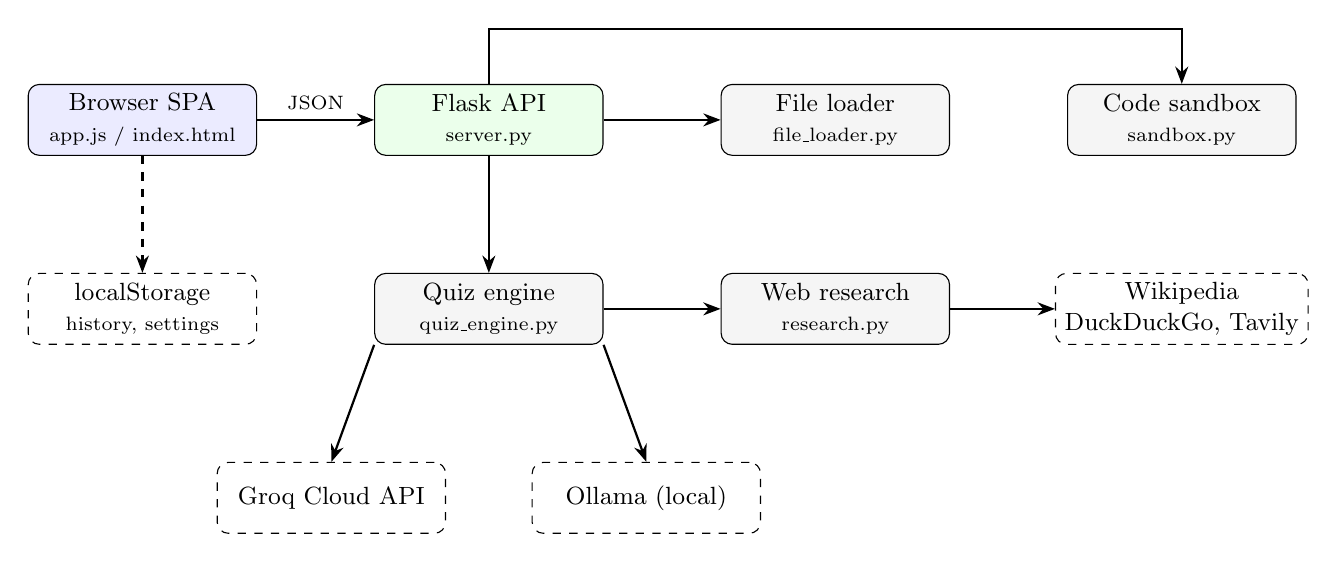
\begin{tikzpicture}[
    box/.style={draw, rounded corners, minimum width=2.9cm, minimum height=0.9cm, align=center, font=\small, fill=gray!8},
    ext/.style={draw, dashed, rounded corners, minimum width=2.9cm, minimum height=0.9cm, align=center, font=\small},
    arr/.style={-{Stealth[length=2.2mm]}, thick}
]
\node[box, fill=blue!8]  (ui)  at (0,0)       {Browser SPA\\ \scriptsize app.js / index.html};
\node[box, fill=green!8] (api) at (4.4,0)     {Flask API\\ \scriptsize server.py};
\node[box]               (fl)  at (8.8,0)     {File loader\\ \scriptsize file\_loader.py};
\node[box]               (sb)  at (13.2,0)    {Code sandbox\\ \scriptsize sandbox.py};
\node[ext]               (ls)  at (0,-2.4)    {localStorage\\ \scriptsize history, settings};
\node[box]               (eng) at (4.4,-2.4)  {Quiz engine\\ \scriptsize quiz\_engine.py};
\node[box]               (res) at (8.8,-2.4)  {Web research\\ \scriptsize research.py};
\node[ext]               (web) at (13.2,-2.4) {Wikipedia\\ DuckDuckGo, Tavily};
\node[ext]               (groq) at (2.4,-4.8) {Groq Cloud API};
\node[ext]               (oll)  at (6.4,-4.8) {Ollama (local)};

\draw[arr] (ui) -- node[above, font=\scriptsize]{JSON} (api);
\draw[arr, dashed] (ui) -- (ls);
\draw[arr] (api) -- (eng);
\draw[arr] (api) -- (fl);
\draw[arr] (api.north) -- ++(0,0.7) -| (sb.north);
\draw[arr] (eng) -- (res);
\draw[arr] (res) -- (web);
\draw[arr] (eng.south west) -- (groq.north);
\draw[arr] (eng.south east) -- (oll.north);
\end{tikzpicture}
\caption{High-level system architecture of Recall}
\label{fig:arch}
\end{figure}

\section{Data Flow Diagram (DFD) Hierarchy}
\subsection{Level 0 -- context}
The learner supplies a topic or files and settings; the system returns a structured quiz, feedback on answers and exportable results. External entities are the LLM provider (Groq or Ollama) and the web sources used for research.

\subsection{Level 1 -- main processes}
\begin{figure}[H]
\centering
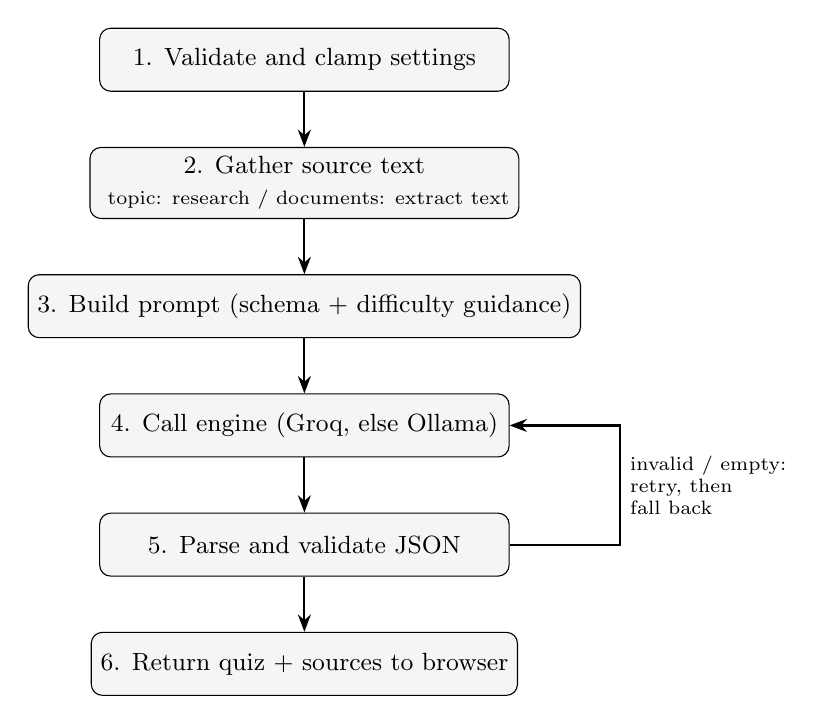
\begin{tikzpicture}[
    node distance=0.7cm,
    proc/.style={draw, rounded corners, minimum width=5.2cm, minimum height=0.8cm, align=center, font=\small, fill=gray!8},
    arr/.style={-{Stealth[length=2.2mm]}, thick}
]
\node[proc] (a) {1. Validate and clamp settings};
\node[proc, below=of a] (b) {2. Gather source text\\\ \scriptsize topic: research / documents: extract text};
\node[proc, below=of b] (c) {3. Build prompt (schema + difficulty guidance)};
\node[proc, below=of c] (d) {4. Call engine (Groq, else Ollama)};
\node[proc, below=of d] (e) {5. Parse and validate JSON};
\node[proc, below=of e] (f) {6. Return quiz + sources to browser};
\foreach \s/\t in {a/b,b/c,c/d,d/e,e/f} \draw[arr] (\s) -- (\t);
\draw[arr] (e.east) -- ++(1.4,0) |- node[pos=0.25, right, font=\scriptsize, align=left]{invalid / empty:\\retry, then\\fall back} (d.east);
\end{tikzpicture}
\caption{Level-1 data flow for quiz generation}
\label{fig:dfd1}
\end{figure}

\section{Explicit Technology Stack Justification}
\begin{table}[H]
\centering
\begin{tabularx}{\textwidth}{@{} p{3.2cm} p{3.4cm} X @{}}
\toprule
\textbf{Layer} & \textbf{Technology} & \textbf{Justification} \\
\midrule
Web server & Flask (Python) & Minimal, easy to read, ideal for a small JSON API and static hosting. \\
Front end & HTML, CSS, vanilla JavaScript & No build step; the whole UI is three static files served by Flask. \\
Cloud LLM & Groq chat-completions API & Very low latency; supports JSON-object response mode. \\
Local LLM & Ollama (default \texttt{llama3.2:3b}) & Works offline and without an API key. \\
Research & Wikipedia API, DuckDuckGo instant answer, Tavily & Free, no key needed except Tavily (optional). \\
Documents & pypdf, python-docx, python-pptx & Pure-Python text extraction for the supported formats. \\
Configuration & python-dotenv & Keeps keys out of source code. \\
Legacy UI & Streamlit & The earlier prototype is kept in \texttt{legacy\_streamlit/}. \\
\bottomrule
\end{tabularx}
\caption{Technology stack}
\label{tab:stack}
\end{table}

\chapter{Backend Development \& API Design}

\section{Introduction to the API Ecosystem}
The back end is a single Flask application (\texttt{recall/server.py}) that serves the static front end at \texttt{/} and exposes six JSON endpoints under \texttt{/api}. The server is started with \texttt{python -m recall.server}, binds to \texttt{127.0.0.1} and reads the port from the \texttt{PORT} environment variable (default 8000). Uploads are limited to 40~MB through Flask's \texttt{MAX\_CONTENT\_LENGTH}, and an error handler returns a readable JSON message for HTTP 413.

\section{Settings Validation and Error Handling}
All quiz settings arriving from the browser are passed through one function, \texttt{\_settings()}, which clamps numbers to safe ranges and replaces unknown values with defaults. This centralisation means no endpoint can request, for example, 500 questions or an unsupported difficulty.

\begin{table}[H]
\centering
\begin{tabularx}{\textwidth}{@{} p{3cm} p{3.6cm} X @{}}
\toprule
\textbf{Setting} & \textbf{Allowed values} & \textbf{Default / behaviour} \\
\midrule
\texttt{difficulty} & Easy, Medium, Hard & Medium \\
\texttt{n\_mcq} & 0--20 & 5 \\
\texttt{n\_short} & 0--10 & 2 \\
\texttt{n\_code} & 0--5 & 0 \\
\texttt{language} & Python, Java, C, C++, JavaScript & Python \\
\texttt{engine} & auto, groq, ollama & auto \\
Total questions & at least 1 & otherwise a \texttt{ValueError} is raised \\
\bottomrule
\end{tabularx}
\caption{Clamped quiz settings}
\label{tab:settings}
\end{table}

Errors follow a uniform contract: a \texttt{ValueError} (bad user input) becomes HTTP~400 with \texttt{\{"error": "..."\}}, and any other exception (engine failure, network error) becomes HTTP~502.

\section{API Endpoint Reference}
\begin{table}[H]
\centering
\begin{tabularx}{\textwidth}{@{} p{1.6cm} p{4.6cm} X @{}}
\toprule
\textbf{Method} & \textbf{Path} & \textbf{Purpose and body} \\
\midrule
GET  & \texttt{/api/status} & Lists available engines and capabilities (web research, Tavily, documents, code runner, AI grading). \\
POST & \texttt{/api/quiz/topic} & JSON: \texttt{topic, use\_web, depth, difficulty, n\_mcq, n\_short, n\_code, language, engine}. Returns \texttt{quiz, sources, web\_used}. \\
POST & \texttt{/api/quiz/document} & Multipart: \texttt{files[]}, \texttt{text}, \texttt{settings} (JSON string). Returns \texttt{quiz, files, chars}. \\
POST & \texttt{/api/grade} & JSON: \texttt{answer, model\_answer, key\_points}. Returns \texttt{score, hits, misses, feedback}. \\
POST & \texttt{/api/run} & JSON: \texttt{code, test\_cases, language}. Returns pass/fail counts and per-case results. \\
POST & \texttt{/api/export/markdown} & JSON: \texttt{quiz, difficulty}. Returns the quiz as Markdown text. \\
\bottomrule
\end{tabularx}
\caption{API endpoints}
\label{tab:endpoints}
\end{table}

\section{Data Dictionary \& Contract Payload Specifications}
\subsection{Quiz object}
A quiz is an object with three arrays, any of which may be empty.
\begin{lstlisting}[language=JSON, caption={Quiz payload returned by the generation endpoints}, label={lst:quiz-json}]
{
  "mcq":    [{ "question": "...", "options": ["A","B","C","D"],
               "answer_index": 2, "explanation": "...",
               "source_quote": "..." }],
  "short":  [{ "question": "...", "model_answer": "...",
               "key_points": ["...", "..."] }],
  "coding": [{ "question": "...", "language": "Python",
               "starter_code": "...", "solution": "...",
               "test_cases": [{ "input": "3\n", "expected_output": "6" }],
               "explanation": "..." }]
}
\end{lstlisting}

\subsection{Grading result}
\begin{lstlisting}[language=JSON, caption={Response of the grading endpoint}, label={lst:grade-json}]
{ "score": 70, "hits": ["defined the term"],
  "misses": ["did not mention complexity"],
  "feedback": "Good start; add the time complexity." }
\end{lstlisting}

\section{Document Quiz Endpoint Flow}
For \texttt{/api/quiz/document} the server reads the settings, collects pasted text, rejects any file whose extension is not in the allowed set (\texttt{pdf, docx, pptx, txt, md}), extracts text from each file, joins everything and calls the quiz engine. The response also reports the file names and total character count so the interface can confirm what was read.

\screenshot{api_status}{Response of the \texttt{/api/status} endpoint shown in the browser, listing the available engines and capabilities}{fig:api-status}{Open http://localhost:8000/api/status in the browser and capture the JSON.}

\chapter{AI Quiz Generation Engine}

\section{Pipeline Architecture and Operational Overview}
The module \texttt{recall/quiz\_engine.py} is the core of the system. It converts a request into a prompt, sends the prompt to an engine, and converts the reply into a validated quiz. The same pipeline serves document quizzes, topic quizzes and answer grading.

\section{Algorithmic Execution Flowchart}
\begin{figure}[H]
\centering
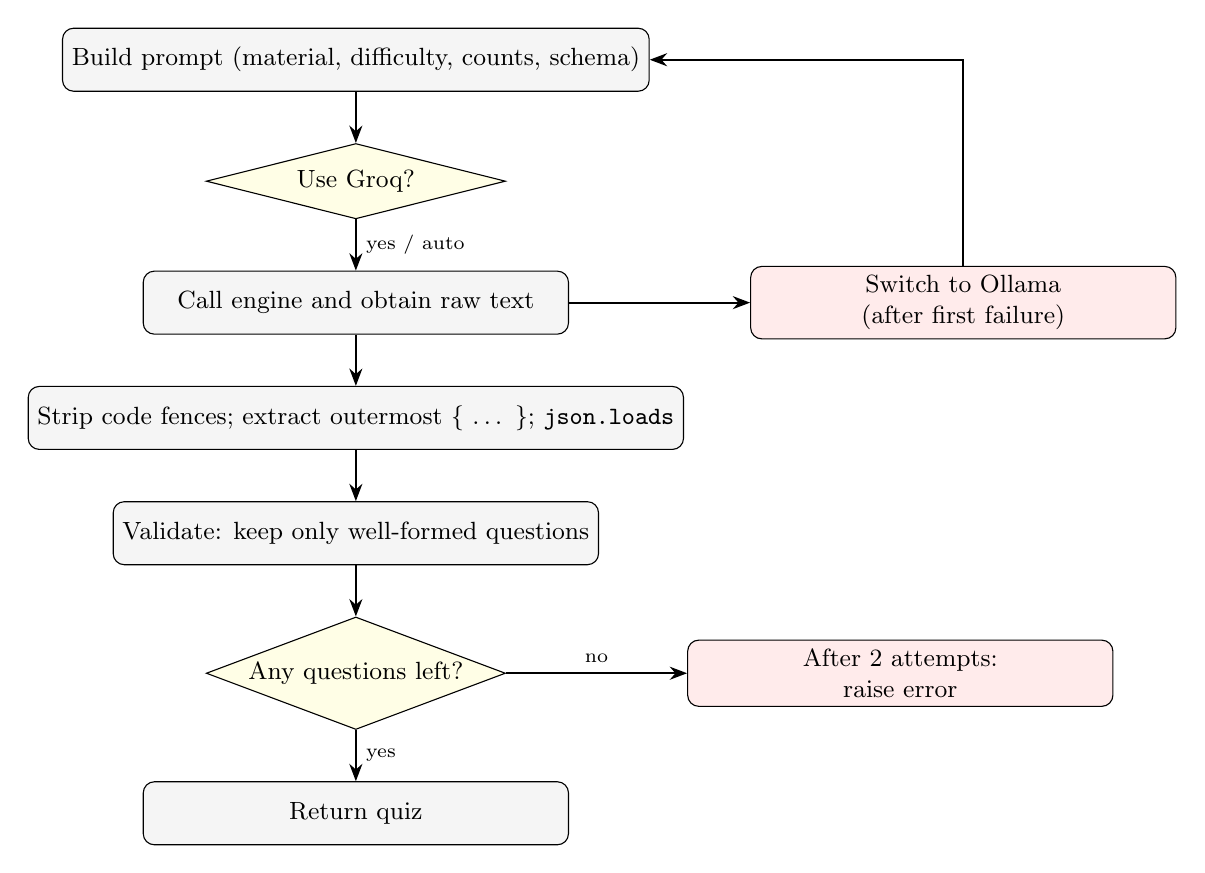
\begin{tikzpicture}[
    node distance=0.65cm,
    st/.style={draw, rounded corners, minimum width=5.4cm, minimum height=0.8cm, align=center, font=\small, fill=gray!8},
    dc/.style={draw, diamond, aspect=2.6, minimum width=3.8cm, align=center, font=\small, fill=yellow!10, inner sep=1pt},
    arr/.style={-{Stealth[length=2.2mm]}, thick}
]
\node[st] (p) {Build prompt (material, difficulty, counts, schema)};
\node[dc, below=of p] (g) {Use Groq?};
\node[st, below=of g] (call) {Call engine and obtain raw text};
\node[st, below=of call] (parse) {Strip code fences; extract outermost \{ \dots\ \}; \texttt{json.loads}};
\node[st, below=of parse] (val) {Validate: keep only well-formed questions};
\node[dc, below=of val] (any) {Any questions left?};
\node[st, below=of any] (ok) {Return quiz};
\node[st, right=2.3cm of call, fill=red!8] (fb) {Switch to Ollama\\ (after first failure)};
\node[st, right=2.3cm of any, fill=red!8] (err) {After 2 attempts:\\ raise error};

\draw[arr] (p) -- (g);
\draw[arr] (g) -- node[right, font=\scriptsize]{yes / auto} (call);
\draw[arr] (call) -- (parse);
\draw[arr] (parse) -- (val);
\draw[arr] (val) -- (any);
\draw[arr] (any) -- node[right, font=\scriptsize]{yes} (ok);
\draw[arr] (any.east) -- node[above, font=\scriptsize]{no} (err.west);
\draw[arr] (call.east) -- (fb.west);
\draw[arr] (fb.north) |- (p.east);
\end{tikzpicture}
\caption{Quiz generation and validation flow}
\label{fig:gen-flow}
\end{figure}

\section{Prompt Design}
Two system prompts are used. The document prompt instructs the model to act as a university examiner and to create questions \textit{only} from the provided material; the topic prompt allows well-established knowledge when no web material is available but forbids inventing facts. Both require a single JSON object with no markdown fences. The user prompt carries four ingredients:
\begin{enumerate}
\item the \textbf{difficulty guidance} string (Easy: recall and definitions; Medium: application with plausible distractors; Hard: multi-step analysis and edge cases);
\item the \textbf{question counts} for each type, with an instruction to return an empty list for any type whose count is zero;
\item the \textbf{JSON schema} (Listing~\ref{lst:quiz-json});
\item the \textbf{material}, truncated to 30{,}000 characters for the cloud engine or 10{,}000 for the local engine to respect its context window.
\end{enumerate}
The complete prompt text is reproduced in Appendix~\ref{app:prompts}.

\section{Parsing and Validation}
Models occasionally wrap JSON in prose or code fences. The parser removes fences, locates the first \texttt{\{} and the last \texttt{\}}, and decodes the slice. Validation then filters each category:
\begin{itemize}
\item an MCQ is kept only if it has exactly four options and an \texttt{answer\_index} from 0 to 3;
\item a written question needs both a question and a model answer;
\item a coding question needs both a question and a reference solution.
\end{itemize}
A reply that yields no valid questions is treated as a failure.

\section{Engines and Fallback Strategy}
\begin{table}[H]
\centering
\begin{tabularx}{\textwidth}{@{} p{2.4cm} p{4.4cm} X @{}}
\toprule
\textbf{Engine} & \textbf{Selection} & \textbf{Details} \\
\midrule
Groq Cloud & \texttt{engine=groq}, or \texttt{auto} when \texttt{GROQ\_API\_KEY} starts with \texttt{gsk\_} & HTTPS call to the chat-completions endpoint with \texttt{response\_format=json\_object}, temperature 0.3, 45~s time-out. \\
Ollama & \texttt{engine=ollama}, or \texttt{auto} without a key & Local model (default \texttt{llama3.2:3b}) called through the \texttt{ollama} package in JSON mode. \\
\bottomrule
\end{tabularx}
\caption{Supported engines}
\label{tab:engines}
\end{table}
The function \texttt{\_run\_prompt} makes up to two attempts. If the first attempt with the cloud engine fails for any reason, the second attempt uses the local engine. After two failures a descriptive error is raised, which the server turns into HTTP~502.

\section{AI Grading of Written Answers}
\texttt{grade\_short\_answer} sends the model answer, the key points and the student's answer to the engine and asks for a JSON object with \texttt{score} (0--100), \texttt{hits}, \texttt{misses} and \texttt{feedback}, using temperature 0.2 for consistency. If grading fails, a neutral result (score~0, all key points listed as missed, and a message asking the learner to compare with the model answer) is returned so that the quiz can continue.

\section{Markdown Export}
\texttt{to\_markdown} renders a quiz as Markdown: numbered MCQs with lettered options, the answer line with explanation and optional source quote, model answers for written questions and reference solutions in fenced code blocks.

\screenshot{loading_generation}{Generation in progress: the loading view shows the stages ``Searching the web'', ``Reading the best sources'', ``Writing your questions'' and ``Checking answers''}{fig:loading}{Click Generate on the home page and capture the animated loading screen with its step list.}

\screenshot{ai_grading}{AI grading of a written answer: score, overall feedback, key points covered (green) and missed (red)}{fig:ai-grading}{Answer a written question and press ``Check with AI''.}

\chapter{Web Research and Document Ingestion}

\section{Purpose}
Both quiz types need \textit{source material}. For topic quizzes it is gathered from the web by \texttt{recall/research.py}; for document quizzes it is extracted from uploaded files by \texttt{recall/file\_loader.py}. Supplying real text to the model is what allows questions to be grounded and attributed.

\section{Web Research Pipeline}
\subsection{Sources}
\begin{table}[H]
\centering
\begin{tabularx}{\textwidth}{@{} p{2.6cm} p{3cm} X @{}}
\toprule
\textbf{Source} & \textbf{Availability} & \textbf{What is retrieved} \\
\midrule
Tavily & Only if \texttt{TAVILY\_API\_KEY} is set & Advanced web search; content snippets of the top results. \\
Wikipedia & Always, no key & Search for the topic, then plain-text extracts of the top articles (references and external-link sections removed). \\
DuckDuckGo & Always, no key & Instant-answer abstract and a few related-topic lines. \\
\bottomrule
\end{tabularx}
\caption{Research sources}
\label{tab:sources}
\end{table}

\subsection{Depth levels}
The learner chooses a research depth that controls how many Wikipedia pages are fetched and how much text is kept per page.
\begin{table}[H]
\centering
\begin{tabularx}{\textwidth}{@{} p{2.5cm} p{3.2cm} X @{}}
\toprule
\textbf{Depth} & \textbf{Wikipedia pages} & \textbf{Characters per page} \\
\midrule
Quick & 1 & 7{,}000 \\
Standard (default) & 3 & 7{,}000 \\
Deep & 5 & 9{,}000 \\
\bottomrule
\end{tabularx}
\caption{Research depth}
\label{tab:depth}
\end{table}

\subsection{Concurrent retrieval and fault tolerance}
The three sources are queried in parallel with a thread pool of three workers and a 12-second time-out each. A failure in any single source (network blocked, time-out, malformed JSON) is caught, recorded in an \texttt{errors} list and ignored; the remaining sources are still used. Results are de-duplicated by URL and concatenated into one block of the form \texttt{\#\#\# SOURCE n: title (site)} followed by its text, capped at 30{,}000 characters. The list of titles and links is returned separately and displayed on the results page.

\begin{lstlisting}[style=pseudo, caption={Simplified logic of the research function}, label={lst:research}]
research(topic, depth):
    pages <- {quick: 1, standard: 3, deep: 5}[depth]
    run in parallel: tavily(topic), wikipedia(topic, pages), duckduckgo(topic)
    for each source: on error -> record error, use empty list
    docs <- merge results in order tavily, wikipedia, duckduckgo
    drop duplicate URLs
    material <- "### SOURCE i: title (site)" + text for each doc, cut at 30000 chars
    return material, sources, errors
\end{lstlisting}

\subsection{Offline behaviour}
If every source fails, the material is empty and the engine is told to rely on its own reliable knowledge. The response sets \texttt{web\_used=false} and the interface shows a notice so the learner knows the questions are not source-backed.

\screenshot{topic_sources}{Results page of a topic quiz listing the web sources used to ground the questions}{fig:sources}{Finish a topic quiz with ``Research the web'' enabled and capture the Sources list on the results page.}

\section{Document Ingestion}
\texttt{extract\_text(name, bytes)} dispatches on the file extension.
\begin{table}[H]
\centering
\begin{tabularx}{\textwidth}{@{} p{2cm} p{3.2cm} X @{}}
\toprule
\textbf{Format} & \textbf{Library} & \textbf{Extraction rule} \\
\midrule
PDF & pypdf & Text of every page, joined by newlines. \\
DOCX & python-docx & Text of every paragraph. \\
PPTX & python-pptx & Text frames of all shapes on every slide. \\
TXT, MD & built-in & Decoded as UTF-8, ignoring invalid bytes. \\
\bottomrule
\end{tabularx}
\caption{Supported document formats}
\label{tab:formats}
\end{table}
Text from several files and any pasted text is combined. If the combined text contains fewer than 80 characters, generation is refused with a clear message; this protects against empty or scanned (image-only) documents.

\screenshot{docs_upload}{Document tab of the composer with the drag-and-drop zone, file chips and paste area}{fig:docs-upload}{Switch to ``My documents'' on the home page, add one PDF or slide deck and capture the composer.}

\chapter{Code Execution Sandbox}

\section{Purpose and Design}
Coding questions are only useful if the learner can check an answer. \texttt{recall/sandbox.py} provides this by running submitted code against the test cases that accompany each coding question. Each test case consists of a stdin string and the expected stdout.

\section{Execution Model}
For every test case the module performs the following steps:
\begin{enumerate}
\item The code is written to a temporary \texttt{.py} file.
\item It is executed with the same Python interpreter as the server (\texttt{sys.executable}) in a subprocess, with the test input piped to stdin and the environment variable \texttt{PYTHONIOENCODING=utf-8}.
\item Standard output and standard error are captured and truncated to 10{,}000 characters each.
\item The subprocess is limited to a 5-second time-out; on expiry it is terminated and the case is reported as timed out.
\item The temporary file is always removed in a \texttt{finally} block.
\end{enumerate}

\section{Result Evaluation}
A test case passes only if the process did not time out, exited with return code~0 and its trimmed stdout equals the trimmed expected output. For each case the endpoint returns the input, the expected and actual output, a pass flag and an error message (a time-out notice or the last error text from stderr). The response also carries the totals \texttt{passed}, \texttt{failed} and \texttt{total}.

\begin{lstlisting}[style=pseudo, caption={Evaluation of one test case}, label={lst:tc}]
result <- run_code(code, stdin = test.input, timeout = 5s)
actual <- strip(result.stdout)
passed <- (not result.timed_out) and result.returncode == 0
          and actual == strip(test.expected_output)
\end{lstlisting}

\section{Language Support and Limitations}
The user interface lets the learner request coding questions in Python, Java, C, C++ or JavaScript, but \textbf{only Python can currently be executed}; for any other language the runner returns the message ``Only Python execution is supported currently''. The runner is a convenience for local practice and has the following security limits, which are discussed further in Chapter~\ref{chap:security}:
\begin{itemize}
\item the code runs with the same privileges as the server, without file-system or network isolation;
\item only wall-clock time and output size are limited, not memory or CPU.
\end{itemize}
It must therefore never be exposed to untrusted users on a public network.

\screenshot{coding_question}{A coding question with starter code editor and test-case results after pressing Run}{fig:coding}{Generate a quiz with one Python coding question, type or paste a solution, press Run and capture the editor plus the passed/failed test list.}

\chapter{Frontend Engineering \& User Experience}

\section{Introduction}
The front end is a single-page application written in plain HTML, CSS and JavaScript (\texttt{recall/static/index.html}, \texttt{styles.css}, \texttt{app.js}) with no build step and no framework. It uses a ``glass'' visual style on a deep-violet background and is organised as a sidebar, a main work area and a right-hand information rail.

\section{Views and Navigation}
The main area switches between six views: \textbf{Home} (the composer), \textbf{Loading}, \textbf{Quiz}, \textbf{Results}, \textbf{Review} and \textbf{History}. The sidebar offers navigation, a list of recent quizzes with search, and settings. The right rail shows the active AI engine with an engine selector, the server capabilities reported by \texttt{/api/status}, and the learner's activity statistics with a score sparkline.

\screenshot{home}{Home view: composer with topic input, difficulty, mode and question-mix controls, and the capability rail}{fig:home}{Open http://localhost:8000 and capture the whole home page.}

\section{The Composer}
The composer offers two input tabs. \textbf{Any topic} accepts up to 300 characters, a ``Research the web'' switch and a depth selector. \textbf{My documents} provides a drag-and-drop zone, file chips and a paste area. Segmented controls choose difficulty (Easy, Medium, Hard) and mode (Practice or Exam); a popover with steppers sets the number of MCQ, written and coding questions, the coding language and the exam time. \texttt{Ctrl+Enter} generates the quiz.

\screenshot{question_mix}{The question-mix popover with steppers for multiple-choice, written and coding questions, language and exam time}{fig:mix}{Click the mix chip (e.g.\ ``5 MCQ - 2 written'') and capture the open popover.}

\section{Taking a Quiz}
\subsection{Practice mode}
After the learner picks an option the correct answer, explanation and, if available, the source quote are revealed immediately. Written answers can be graded on demand with the \textit{Check with AI} button (or compared with the model answer), and coding answers can be run against test cases with \textit{Run tests}; a \textit{Show solution} button reveals the reference solution.

\subsection{Exam mode}
Exam mode shows a countdown timer, a question grid for jumping between questions, and a flag button to mark questions for review. Feedback is withheld until the quiz is submitted. Keyboard shortcuts are available: keys \texttt{1}--\texttt{4} choose an option, the arrow keys move between questions and \texttt{Enter} advances.

\screenshot{quiz_practice}{Practice-mode question card with immediate feedback, explanation and source quote}{fig:practice}{Take a quiz in Practice mode, answer one MCQ and capture the card with the green/red feedback and explanation.}
\screenshot{quiz_exam}{Exam mode with countdown timer, question grid and flag-for-review control}{fig:exam}{Start a quiz in Exam mode and capture the top of the quiz view showing the timer and question grid.}

\section{Results, Review and the Retry Loop}
On submission the results page shows a score ring with a short verdict, tiles for the percentage score, multiple-choice questions correct, the number of written and coding questions, and the time taken, plus a row of coloured dots showing the status of each question. Action buttons let the learner retry only the mistakes (retry loop), review the mistakes or all questions, retake the quiz, download it as JSON or Markdown, or start a new quiz. For topic quizzes a ``Sources used'' panel lists the web pages the questions were based on. If some questions are left unanswered, a confirmation dialog appears before submission.

\screenshot{results}{Results page with score summary, retry and review actions, export buttons and the list of sources used}{fig:results}{Submit a finished quiz and capture the results page.}
\screenshot{review}{Review of incorrect answers with the correct option and explanation}{fig:review}{On the results page choose the review of mistakes and capture it.}

\section{State, History and Statistics}
All persistent state is stored with the prefix \texttt{recall.} in the browser's \texttt{localStorage}: the learner's name, default engine, optional server address and the list of past quizzes with scores. Reads and writes are wrapped in \texttt{try/catch}, so the application still works when storage is unavailable. The sidebar and the activity panel derive recent quizzes, number of quizzes taken, questions answered and average score from this history; the history view allows searching, re-taking and clearing.

\screenshot{history}{History view listing earlier quizzes with scores, with the activity statistics panel}{fig:history}{After taking two or three quizzes open History from the sidebar and capture it.}

\section{Demo Mode}
On start-up the page calls \texttt{/api/status}. If the server cannot be reached, a banner announces \textit{Demo mode} and a small built-in sample quiz is used, so the interface can still be shown, for example when the static files are hosted without the Flask back end. In demo mode live research, document upload and code execution are unavailable.

\section{Responsive and Accessible Design}
The layout collapses for narrow screens with a menu button for the sidebar. Interactive elements carry ARIA labels, the toast notifications use a polite live region and dialogs use the native \texttt{<dialog>} element for settings and confirmations.

\chapter{Security, Testing \& Deployment}
\label{chap:security}

\section{Security Measures and Data Privacy}
\begin{itemize}
\item \textbf{Secrets.} API keys are read from environment variables loaded from a local \texttt{.env} file. The file is listed in \texttt{.gitignore} and a template, \texttt{.env.example}, with empty placeholders is committed instead.
\item \textbf{Network exposure.} The development server binds to \texttt{127.0.0.1} only, so it is not reachable from other machines.
\item \textbf{Input validation.} Quiz settings are clamped in one function; topic length is limited to 300 characters; the upload extension is checked against a whitelist; total upload size is limited to 40~MB.
\item \textbf{Data minimisation.} The server stores nothing. Quiz history remains in the learner's browser. Only the text needed for generation (topic, extracted material, answers to be graded) is sent to the selected model provider; choosing the Ollama engine keeps this entirely on the local machine.
\item \textbf{Output handling.} Model output is parsed as JSON and filtered through a schema validator before it reaches the interface.
\end{itemize}

\textbf{Known risks.} The code runner executes learner-submitted Python with the server's privileges and offers no isolation from the file system or network (Section~\ref{sec:future-hardening}). The application has no authentication, so it must not be exposed on a public address. These are acceptable for the intended single-user local scenario and are listed as future work.

\section{System Testing}
No automated test suite exists yet. The system was therefore verified by manual black-box testing of the API with \texttt{curl} against a running instance, plus interactive testing of the interface. Table~\ref{tab:tests} records the executed API test cases and their observed results.

\begin{table}[H]
\centering
\small
\begin{tabularx}{\textwidth}{@{} p{0.9cm} p{4.6cm} p{4.4cm} X @{}}
\toprule
\textbf{ID} & \textbf{Test case} & \textbf{Expected} & \textbf{Observed} \\
\midrule
T1 & GET \texttt{/api/status} & HTTP 200, engines and capabilities & Pass: 200, two engines listed \\
T2 & Topic quiz with empty topic & HTTP 400, message asking for a topic & Pass \\
T3 & Topic quiz with 0 MCQ, 0 written, 0 coding & HTTP 400, ``Choose at least one question.'' & Pass \\
T4 & Run correct doubling program on 2 cases & 2 passed, 0 failed & Pass \\
T5 & Run program printing wrong output & 1 failed with actual and expected shown & Pass \\
T6 & Run infinite loop & Terminated; ``timed out after 5 seconds'' & Pass (about 5.0~s) \\
T7 & Upload a file named \texttt{bad.exe} & HTTP 400, unsupported file type & Pass \\
T8 & Document quiz with fewer than 80 characters & HTTP 400, not enough text & Pass \\
T9 & Grade an empty answer & HTTP 400, ``Write an answer first.'' & Pass \\
T10 & Export a one-question quiz to Markdown & Numbered question, lettered options, answer line & Pass \\
T11 & Topic quiz ``Binary search'', quick depth, Easy, 2 MCQ + 1 written, auto engine & HTTP 200 with valid questions & Pass: valid MCQs returned from the cloud engine \\
\bottomrule
\end{tabularx}
\caption{Executed API test cases}
\label{tab:tests}
\end{table}

\section{Deployment}
\subsection{Local deployment}
\begin{enumerate}
\item Create a virtual environment and install \texttt{requirements.txt}.
\item Copy \texttt{.env.example} to \texttt{.env} and set \texttt{GROQ\_API\_KEY} (optional \texttt{TAVILY\_API\_KEY}); for offline use install Ollama and run \texttt{ollama pull llama3.2:3b}.
\item Start the server with \texttt{python -m recall.server} (or \texttt{scripts/run.bat} on Windows) and open \texttt{http://localhost:8000}.
\end{enumerate}

\subsection{Source control}
The project is published as a public Git repository containing the source, front end, scripts and this report's LaTeX sources, while the environment file, virtual environment and caches are excluded.

\section{Planned Hardening}
\label{sec:future-hardening}
Before any shared or public deployment the code runner should execute inside a container or restricted process with no network, memory and CPU limits and a read-only file system, a production WSGI server should replace the Flask development server, and authentication and rate limiting should be added in front of the model endpoints.


\chapter{Standards Adopted}

\section{Design Standards}
\begin{itemize}
\item \textbf{IEEE Std 830 / ISO/IEC/IEEE 29148} -- structure of the requirements specification in Chapter~3.
\item \textbf{REST conventions} -- resource-style paths under \texttt{/api}, use of HTTP methods and JSON bodies, and meaningful status codes (200, 400, 413, 502).
\item \textbf{JSON (RFC 8259)} -- the only data-interchange format between browser, server and model.
\item \textbf{Responsive and accessible web design} -- semantic HTML, ARIA labels and live regions, native dialogs.
\end{itemize}

\section{Coding Standards}
\begin{itemize}
\item \textbf{PEP 8} naming and layout for Python modules, with type hints and docstrings in the sandbox and research modules.
\item Single-responsibility modules inside the \texttt{recall} package, with relative imports.
\item Configuration through environment variables (twelve-factor style); no secrets in source.
\item Defensive error handling at system boundaries: network calls have time-outs and failures degrade gracefully.
\end{itemize}

\section{Testing Standards}
\begin{itemize}
\item Black-box functional testing of every endpoint, including negative cases (invalid input, unsupported files, time-outs) as recorded in Table~\ref{tab:tests}.
\item Each test case states the input, the expected result and the observed result.
\item Recommended next step: convert the executed cases into an automated \texttt{pytest} suite using Flask's test client, with the LLM call mocked.
\end{itemize}

\chapter{Conclusion \& Future Scope}

\section{Comprehensive Project Summary}
Recall demonstrates that a small, dependency-light application can turn arbitrary topics and study documents into complete, gradable quizzes. Source text is retrieved from the web or extracted from files, wrapped in a schema-constrained prompt, sent to a cloud or local language model, parsed, validated and delivered through an exam-style interface with AI grading and a code runner. The key engineering ideas are: grounding questions in visible sources, never trusting raw model output, always providing a fallback path, and keeping the server stateless.

\section{Current System Limitations}
\begin{itemize}
\item Only Python code can be executed, and the runner is not isolated from the host.
\item No user accounts; history is local to one browser.
\item No optical character recognition for scanned documents.
\item Question quality depends on the chosen model and, for topic quizzes, on the quality of retrieved sources.
\item No automated test suite yet.
\item The default cloud model name in code differs from the one in \texttt{.env.example}; the \texttt{.env} value takes precedence.
\end{itemize}

\section{Objectives Traceability Matrix}
\begin{table}[H]
\centering
\begin{tabularx}{\textwidth}{@{} p{1.3cm} X p{3.6cm} @{}}
\toprule
\textbf{Obj.} & \textbf{Objective (Section 1.3)} & \textbf{Where realised} \\
\midrule
1 & Topic quizzes grounded in web sources & Ch.~7, \texttt{research.py} \\
2 & Quizzes from uploaded documents and pasted text & Ch.~7, \texttt{file\_loader.py} \\
3 & Three question types and three difficulties & Ch.~5, Ch.~6 \\
4 & Strict JSON schema, validation and retry & Ch.~6, \texttt{quiz\_engine.py} \\
5 & Cloud engine with offline local fallback & Ch.~6 \\
6 & AI grading and code execution & Ch.~6, Ch.~8 \\
7 & Practice and Exam modes, history, export & Ch.~9 \\
\bottomrule
\end{tabularx}
\caption{Objectives traceability matrix}
\label{tab:trace}
\end{table}

\section{Future Architectural Enhancements}
\begin{itemize}
\item \textbf{Containerised sandbox} supporting Java, C, C++ and JavaScript with resource limits.
\item \textbf{Automated tests} with \texttt{pytest}, mocked engines and continuous integration.
\item \textbf{Accounts and cloud sync} for history, with spaced-repetition scheduling of missed questions.
\item \textbf{Vector retrieval} (embeddings) for long documents, instead of truncating to the first 30{,}000 characters.
\item \textbf{OCR} for scanned PDFs and images of handwritten notes.
\item \textbf{Question quality checks}, such as a second model pass that verifies each answer against its source quote.
\item \textbf{Teacher mode} for sharing a generated quiz through a link and collecting results.
\item \textbf{Streaming generation} so that questions appear as soon as they are produced.
\end{itemize}


\appendix
\chapter{Project Directory Structure}
The following listing shows the top-level file organisation of the source repository.

\begin{lstlisting}[basicstyle=\ttfamily\footnotesize, caption={Repository directory tree}, label={lst:dir-tree}]
recall-ai-quiz-studio/
|-- README.md
|-- requirements.txt
|-- .env.example
|-- .gitignore
|-- recall/
|   |-- __init__.py
|   |-- server.py          Flask app and JSON API
|   |-- quiz_engine.py     prompts, LLM calls, validation, grading
|   |-- research.py        Wikipedia / DuckDuckGo / Tavily research
|   |-- file_loader.py     PDF / DOCX / PPTX / TXT / MD extraction
|   |-- sandbox.py         Python code runner with test cases
|   `-- static/
|       |-- index.html
|       |-- styles.css
|       `-- app.js
|-- legacy_streamlit/
|   |-- app.py
|   |-- theme.py
|   `-- .streamlit/config.toml
|-- scripts/
|   |-- run.bat
|   `-- run.sh
`-- report/
    |-- main.tex
    |-- chapters/
    `-- images/
        |-- KIIT_logo.png
        `-- screenshots/
\end{lstlisting}

\chapter{Prompts and Schema}
\label{app:prompts}

\section{JSON schema given to the model}
\begin{lstlisting}[language=JSON, caption={Schema embedded in every generation prompt}, label={lst:schema}]
{
  "mcq": [{"question": str, "options": [str, str, str, str],
           "answer_index": 0-3, "explanation": str, "source_quote": str}],
  "short": [{"question": str, "model_answer": str, "key_points": [str]}],
  "coding": [{"question": str, "language": str, "starter_code": str,
              "solution": str,
              "test_cases": [{"input": str, "expected_output": str}],
              "explanation": str}]
}
\end{lstlisting}

\section{Difficulty guidance}
\begin{table}[H]
\centering
\begin{tabularx}{\textwidth}{@{} p{2cm} X @{}}
\toprule
\textbf{Level} & \textbf{Guidance placed in the prompt} \\
\midrule
Easy & Recall and definitions; direct facts from the text; obvious distractors. Coding: simple one-concept tasks (loops, conditionals, basic functions). \\
Medium & Understanding and application; small scenarios; plausible distractors. Coding: moderate logic, standard data structures, small algorithms. \\
Hard & Analysis and problem solving; multi-step reasoning, edge cases, subtle distractors. Coding: optimisation, complexity analysis, tricky edge cases. \\
\bottomrule
\end{tabularx}
\caption{Difficulty guidance strings}
\label{tab:difficulty}
\end{table}

\section{System prompts}
\begin{lstlisting}[style=pseudo, caption={Document-quiz system prompt (abridged)}, label={lst:sys-doc}]
You are an expert university examiner for B.Tech Computer Science.
Create quiz questions ONLY from the provided material. For each MCQ,
ensure distractors are plausible and include a source_quote (exact
short excerpt justifying the answer). Respond with a single valid JSON
object and nothing else (no markdown fences).
\end{lstlisting}

\begin{lstlisting}[style=pseudo, caption={Topic-quiz system prompt (abridged)}, label={lst:sys-topic}]
You are an expert university examiner and subject tutor. Create
accurate, well-balanced quiz questions about the requested topic. When
web research material is provided, base questions on it and quote it in
source_quote; otherwise use well-established, uncontroversial knowledge.
Never invent facts. Respond with a single valid JSON object only.
\end{lstlisting}


\end{document}
